%!TEX root = ./HW2.tex

\section{100 Cities}
\subsection{Results}
For 100 cities, the best solution is SA.  EA performs similarly, but has a larger standard deviation.  SA may be better at exploring the state space.  More variety in solution allows it to continue to hone in on a good solution.  The other two methods appear to get stuck in to a local minimum and then have trouble making large improvements from that solution.  The large exploratin also explains the steep decreasing slope for SA.


\begin{table}[H]
\centering
\begin{tabular}{|c|c|c|c|c|c|}
\hline
Algorithm               & \begin{tabular}[c]{@{}c@{}}Total Solutions\\ Generated\end{tabular} & \begin{tabular}[c]{@{}c@{}}Average Min\\ Distance\end{tabular} & St Dev & \begin{tabular}[c]{@{}c@{}}Average\\ Run Time (s)\end{tabular} & St Dev  \\ \hline
Simulated Annealing     & 10,000                                                              & 51,846                                                         & 1993  & 4.79e-6                                                        & 4.32e-7 \\ \hline
Evolutionary Algorithm  & 10,000                                                              & 57,985                                                         & 1886  & 127.00                                                           & 0.47    \\ \hline
Monte Carlo Tree Search & 10,000                                                              & 63,638                                                         & 1865    & 18.70                                                           & 0.59    \\ \hline
\end{tabular}
\caption{Comparison of Solution Quality and Run Time for Each Method with 100 Cities}
\label{tab:100Comparison}
\end{table}

% insert image of example solutions found by search

\begin{figure}[H]
	\centering
    \begin{minipage}{0.45\textwidth}
        \centering
        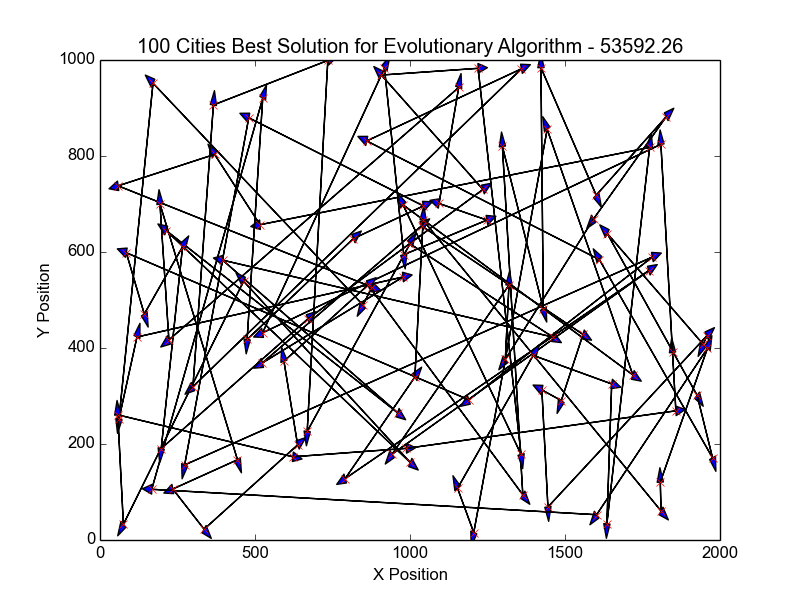
\includegraphics[width=0.9\textwidth]{100City_EA.png} % first figure itself
        \caption{Best Solution for 100 Cities with Evolutionary Algorithm}
        \label{fig:100city_EA}
    \end{minipage}\hfill
    \begin{minipage}{0.45\textwidth}
        \centering
        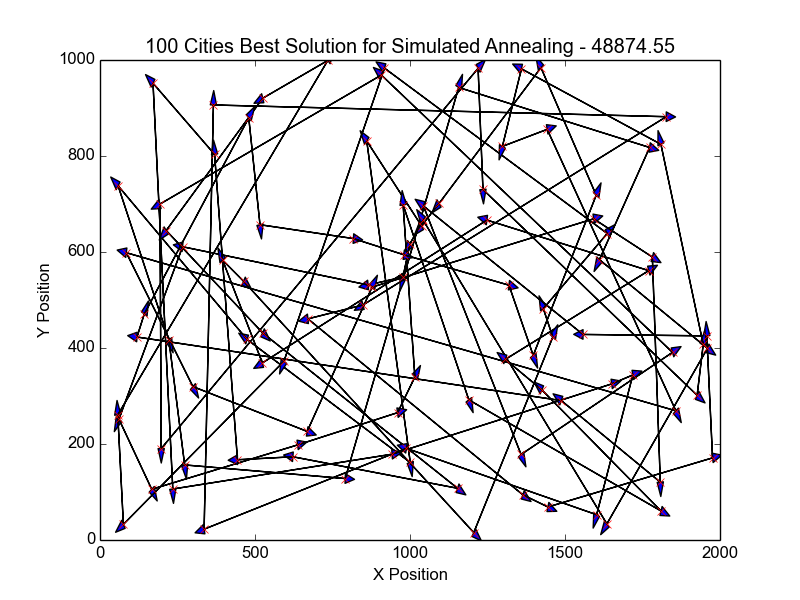
\includegraphics[width=0.9\textwidth]{100City_SA.png} % second figure itself
        \caption{Best Solution for 100 Cities with Simulated Annealing}
        \label{fig:100city_SA}
    \end{minipage}\hfill
    \begin{minipage}{0.45\textwidth}
        \centering
        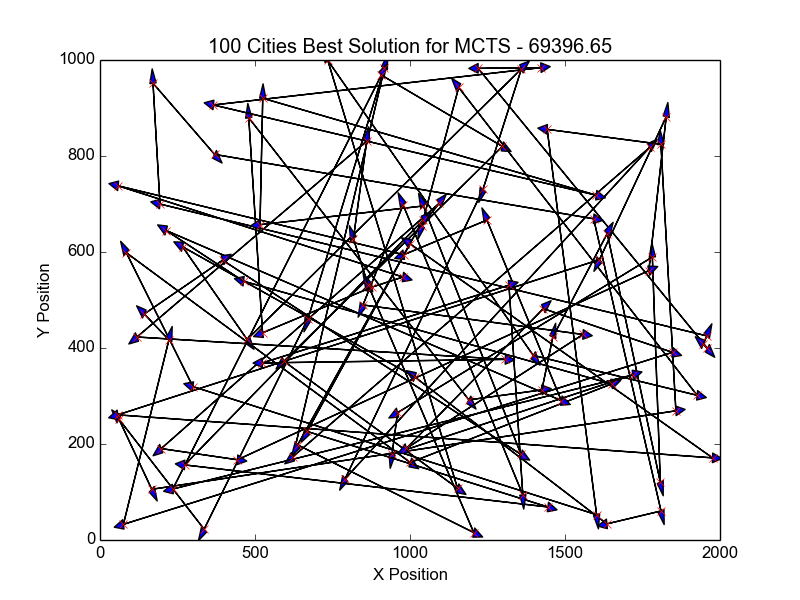
\includegraphics[width=0.9\textwidth]{100City_MCTS.png} % third figure itself
        \caption{Best Solution for 100 Cities with MCTS}
        \label{fig:100city_MCTS}
    \end{minipage}\hfill
    \begin{minipage}{0.45\textwidth}
		\centering
		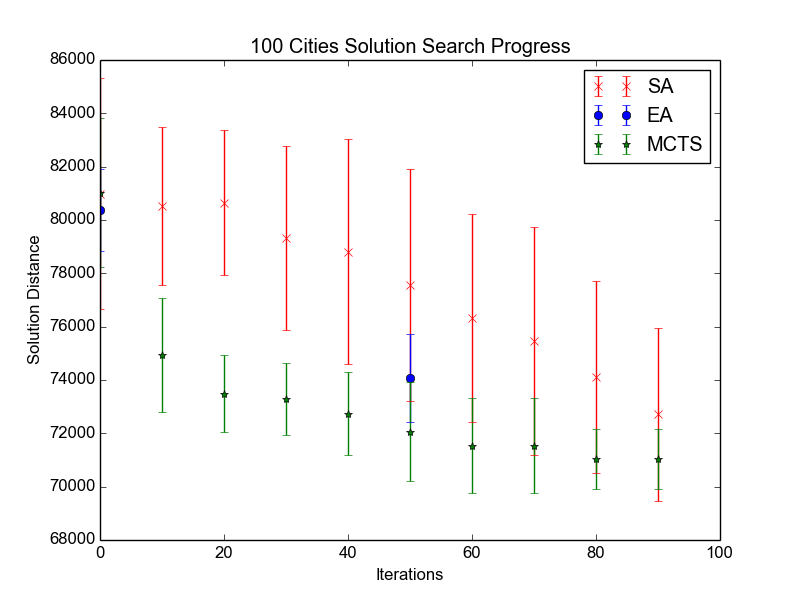
\includegraphics[width=0.9\textwidth]{100City_Solutions.png}
		\caption{Solution Progression for 100 Cities}
		\label{fig:100city_Solution}
    \end{minipage}\hfill
\end{figure}

